\documentclass{beamer}

\usepackage{beamerthemeAmsterdam}
%\usecolortheme{lily}

% PACKAGES
\usepackage[utf8]{inputenc}
\usepackage[francais]{babel}
\usepackage{xcolor}
\usepackage{fancyvrb}
\usepackage{graphicx}
% --

\title{Projet NachOS}

\author{
  Groupe F \newline{}
  {\rule{5cm}{0.4pt}}\newline{}
  Jérémy Derdaele\newline{}
  José-Paul Dominguez\newline{}
  Timothée Frappé--Vialatoux\newline{}
  Nizâmouddine Gangat\newline{}
  {\rule{5cm}{0.4pt}}\newline{}
}

\begin{document}
\begin{frame}
  \titlepage
\end{frame}

\section*{int main(void)}
\begin{frame}
  \frametitle{Sommaire}
  \tableofcontents
\end{frame}

\section{Threads utilisateurs}
\subsection{Propriétés}
\begin{frame}
  \frametitle{Propriétés}
  Les threads utilisateurs:
  \begin{itemize}
  \item Partagent le même espace mémoire
  \item Pas de hiérarchie entre les threads
  \item Identification unique (tid)
  \item Terminaison automatique
  \end{itemize}
\end{frame}

\begin{frame}
  \frametitle{Espace mémoire}
  \begin{center}
    
\includegraphics[scale=0.4]{user_threads.png}
  \end{center}
\end{frame}

\begin{frame}[fragile]
  \frametitle{Création}
\begin{verbatim}
int UserThreadCreate(void (*f)(void*), void* arg);
\end{verbatim}
\begin{itemize}
  \item Alloue une pile pour le nouveau thread
  \item Valeur de retour:
    \begin{itemize}
    \item Succès: un identifiant unique du thread créé
    \item Echec: -1
    \end{itemize}
\end{itemize}
\end{frame}

\begin{frame}[fragile]
  \frametitle{Terminaison}
\begin{verbatim}
void UserThreadExit(void);
\end{verbatim}
\begin{itemize}
  \item Termine immédiatement l'exécution du thread appelant
  \item Le thread 0 peut se terminer avant les autres
  \item Ne libère pas la pile et le tid
\end{itemize}
\end{frame}

\begin{frame}[fragile]
  \frametitle{Attente de Terminaison}
\begin{verbatim}
void UserThreadJoin(int tid);
\end{verbatim}
\begin{itemize}
  \item Attend la terminaison d'un thread, appel bloquant
  \item Si le thread est déjà terminé, l'appel est non bloquant
  \item Permet de libérer la pile allouée et le tid
\end{itemize}
\end{frame}

\section{Mémoire virtuelle}

\begin{frame}
  \frametitle{Processus}
\end{frame}

\subsection{Processus}
\begin{frame}
  \frametitle{Processus : propriétés}
  \begin{itemize}
  \item Espace d'addressage indépendants
  \item Identifié par un id (pid)
  \item Organisation hiérachique
    \begin{itemize}
    \item Un processus ``Père'' crée un processus ``Fils''
    \item Un processus ``Père'' peut attendre la terminaison d'un ``Fils''
    \end{itemize}
  \end{itemize}
\end{frame}

\begin{frame}[fragile]
  \frametitle{Terminaison}
\begin{verbatim}
void Exit(int code);
\end{verbatim}
  \begin{itemize}
  \item Termine immédiatement l'exécution du processus
    \item Tue tout les threads utilisateur
  \end{itemize}
\end{frame}

\begin{frame}[fragile]
  \frametitle{Fork}
\begin{verbatim}
int Fork(void);
\end{verbatim}
Valeur de retour
\begin{itemize}
\item Processus père
  \begin{itemize}
  \item Succès: le pid du fils
  \item Echec: -1
  \end{itemize}
\item Processus fils: Toujours 0
\end{itemize}

Sémantique
\begin{itemize}
\item On duplique entièrement la mémoire du père
\item Certaines pages ne sont jamais modifiées
\end{itemize}
Approche peu efficace
\end{frame}

\begin{frame}
  \frametitle{Copy on Write}
  Lors du Fork:
  \begin{itemize}
    \item On marques toutes les pages du père et du fils en lecture seule
  \end{itemize}

  \begin{center}
  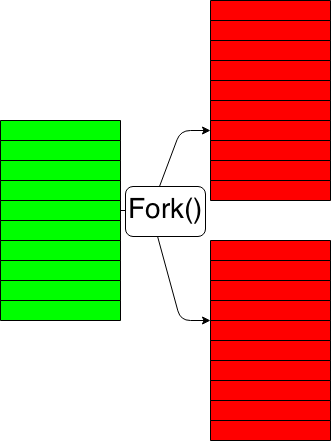
\includegraphics[scale=0.3]{fork_mem.png}
  \end{center}
\end{frame}

\begin{frame}
  \frametitle{Copy on Write}
  Lors d'une exception ReadOnly
  \begin{itemize}
  \item On vérifie que le processus à la permission d'écire
  \item On duplique la page concernée avec permission d'écrire
  \end{itemize}

  \begin{center}
  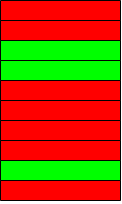
\includegraphics[scale=0.5]{cow.png}
  \end{center}
\end{frame}

\begin{frame}
  \frametitle{Copy on Write}
  Chaque page:
  \begin{itemize}
  \item Peut être référencée par plusieurs processus
  \item Doit être libérée uniquement quand plus aucun processus ne l'utilise
  \end{itemize}
\end{frame}

\begin{frame}[fragile]
  \frametitle{Exec}
\begin{verbatim}
int Exec(const char *filename);
\end{verbatim}
L'espace d'adressage du processus est totalement remplacé par l'executable filename.\\

Valeur de retour
\begin{itemize}
  \item Succès: ne retourne pas car l'espace mémoire est remplacé
  \item Echec: -1
\end{itemize}
\end{frame}

\begin{frame}[fragile]
  \frametitle{ForkExec}
\begin{verbatim}
int ForkExec(const char *filename);
\end{verbatim}
Fork suivi d'un exec mais de manière atomique.
Valeur de retour (pour le père uniquement):
\begin{itemize}
\item Succès: le pid du fils
\item Echec: -1
\end{itemize}
\end{frame}

\begin{frame}
  \frametitle{Terminaison}
  \begin{itemize}
    \item Si un père se termine avant son fils, il est rattaché à ``init'' (pid 1)
    \item Un processus peut attendre la terminaison de son fils avec l'appel système \texttt{int WaitPid(int pid)}
  \end{itemize}

\end{frame}


\subsection{Allocation dynamique}

\begin{frame}
  \frametitle{Mémoire dynamique}
\end{frame}

\begin{frame}
\frametitle{Tas}
\begin{center}
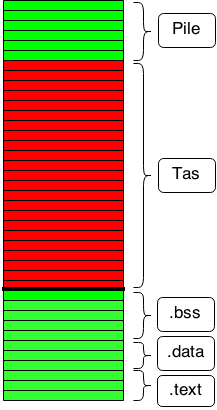
\includegraphics[scale=0.4]{tas.png}
\end{center}
\end{frame}

\begin{frame}
\frametitle{Srbk}
\begin{center}
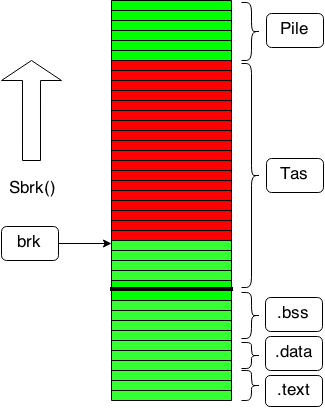
\includegraphics[scale=0.4]{sbrk.png}
\end{center}
\end{frame}

\begin{frame}
  \frametitle{Allocateur de mémoire dynamique}
  Allocateur basé sur des ``free-list''\\

  Primitive:
  \begin{itemize}
    \item void *malloc(size\_t size);
    \item void free(void *ptr);
    \item void *calloc(size\_t nmemb, size\_t size);
    \item void *realloc(void *ptr, size\_t size);
  \end{itemize}
\end{frame}

\begin{frame}[fragile]
  \frametitle{Interpréteur Crisp}
  Un dialecte de Lisp\\
  Objectifs:
  \begin{itemize}
  \item Tester notre système sur une application ``réelle''
  \item Implanter des parties de la librairie standard du C
  \item Bénéficier d'un language de programmation (turing complet)
  \end{itemize}

  {\scriptsize
\begin{verbatim}
{define fact
    {lambda {x}
        {if { = x 0}
            1
            {* x {fact {- x 1}}}
        }
    }
}
\end{verbatim}
}
\end{frame}

\begin{frame}
  \frametitle{Bibliothèque standard C}
  Des parties de la libc sont disponibles à l'utilisateur.

  \begin{itemize}
    \item assert.h: macro assert
    \item ctype.h: tests sur le type d'un caractère
    \item stddef.h: définit NULL, size\_t, etc
    \item stdlib.h: abort(), allocation dynamique
    \item string.h: manipulation de chaines
  \end{itemize}
\end{frame}

\section{Système de fichier}
\subsection{Sémantique}

\begin{frame}
  \frametitle{Système de fichier}
\end{frame}


\begin{frame}
  \frametitle{Présentation}
  \begin{itemize}
  \item Identification des fichiers par des tags
  \item Pas de notion de hiérarchie entre les fichiers
  \item Navigation et gestion grâce aux tags
  \end{itemize}
\end{frame}

\begin{frame}
  \frametitle{Points importants}
  \begin{itemize}
  \item Trouver des fichiers doit être le plus rapide possible
    \begin{itemize}
      \item A partir d'un ensemble de tags
      \item Possibilité d'exclure facilement des tags
    \end{itemize}
  \item Minimiser la taille du système de fichier sur le disque
  \end{itemize}
\end{frame}

\subsection{Implantation}
\begin{frame}
  \frametitle{Structure de données}
  \begin{center}
  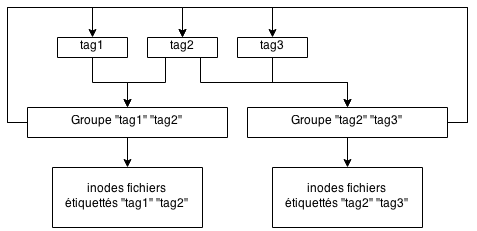
\includegraphics[scale=0.4]{fs_data.png}
  \end{center}
  Structure :
  \begin{itemize}
  \item Groupes composés de tags et des fichiers associés
  \item Les tags référencent les groupes auxquels ils appartiennent
  \end{itemize}
\end{frame}

\begin{frame}
  \frametitle{Structure du disque}
  \begin{center}
  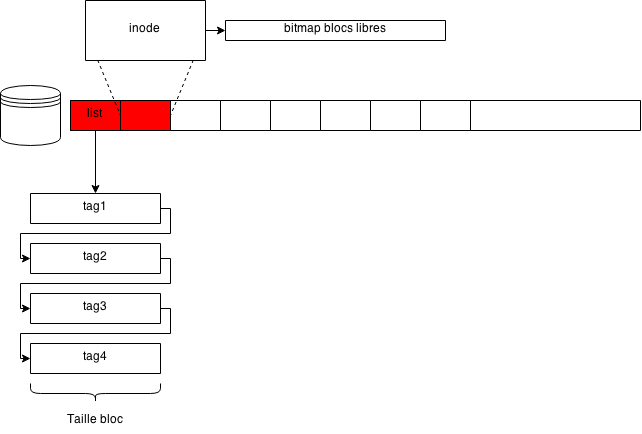
\includegraphics[scale=0.4]{fs_struct.png}
  \end{center}
\end{frame}

\section*{return 0;}

\begin{frame}[fragile]
  \frametitle{Conclusion}
  \begin{itemize}
  \item Améliorations possibles
  \item Déroulement du projet
  \end{itemize}
\begin{verbaterm}[fontsize=\scriptsize]
Questions ?

Ticks: total 869727823, idle 869133578, system 1420, user 592825
Disk I/O: reads 10298, writes 599
Console I/O: reads 354, writes 6
Paging: faults 0
Network I/O: packets received 20, sent 213

Cleaning up...
\end{verbaterm}

\end{frame}

\end{document}
